\documentclass[12pt,a4paper]{article}
\usepackage[margin=1in]{geometry}
\usepackage{graphicx}
\usepackage{float}
\usepackage{booktabs}
\usepackage{array}
\usepackage{longtable}
\usepackage{hyperref}
\usepackage{xcolor}
\usepackage{tikz}
\usetikzlibrary{arrows.meta, positioning, shapes.geometric}

\hypersetup{
    colorlinks=true,
    linkcolor=blue,
    citecolor=blue,
    urlcolor=blue
}

\newcommand{\reservedfigure}[2]{%
\begin{figure}[H]
\centering
\fbox{%
\begin{minipage}[c][0.22\textheight][c]{0.88\textwidth}
\centering
\textbf{Reserved Image Box}\\[0.5em]
#1
\end{minipage}}
\caption{#2}
\end{figure}
}

\newcommand{\reservedwide}[2]{%
\begin{figure}[H]
\centering
\fbox{%
\begin{minipage}[c][0.16\textheight][c]{0.92\textwidth}
\centering
\textbf{Reserved Table or Screenshot Box}\\[0.5em]
#1
\end{minipage}}
\caption{#2}
\end{figure}
}

\title{\textbf{Genetic Algorithm Based Jigsaw Puzzle Solver}\\
\large Project Report}
\author{Coursework Project: \texttt{gaps}}
\date{\today}

\begin{document}
\maketitle

\begin{abstract}
This project implements a coursework-scale solver for Type-1 jigsaw puzzle reconstruction, where puzzle pieces are square, non-overlapping, fixed in orientation, and arranged on a known grid. The work is based on the Genetic Algorithm (GA) approach described by Sholomon, David, and Netanyahu, who introduced an effective GA-based jigsaw solver using a kernel-growing crossover operator and neighbor-based evaluation. In this implementation, an input image can be cropped to a valid piece grid, divided into square pieces, shuffled into a puzzle, and reconstructed by a population-based GA search. The project provides both a command-line interface and a local Streamlit dashboard. The implementation includes deterministic puzzle generation through seeds, manifest-based ground-truth mapping, edge-dissimilarity fitness, roulette selection, elitism, crossover, swap mutation, fitness history tracking, plots, random baselines, generation snapshots, and experiment scripts. Solution quality is evaluated using piece-position accuracy and adjacency accuracy computed from the manifest rather than from raw image bytes. This makes the evaluation reproducible and aligned with the literature distinction between direct comparison and neighbor comparison. The project does not attempt to reproduce the full scale of the reference paper; instead, it demonstrates the main algorithmic ideas in a local, understandable, testable Python system suitable for coursework evaluation.
\end{abstract}

\section{Introduction}
Automatic jigsaw puzzle solving is a combinatorial optimization problem. When an image is cut into many pieces, the number of possible arrangements grows extremely quickly, making brute-force reconstruction infeasible even for moderate piece counts. A solver therefore needs a strategy for searching the space of possible arrangements and a way to judge whether neighboring pieces are likely to belong together.

Genetic Algorithms are suitable for this type of problem because they maintain a population of candidate solutions and improve them over generations. Instead of committing to one greedy decision at a time, a GA can preserve several competing arrangements, select stronger candidates, and combine useful partial structures. Sholomon, David, and Netanyahu proposed an effective GA-based solver for square jigsaw puzzles and introduced a crossover operator that detects and transfers correctly assembled puzzle segments between parent solutions \cite{sholomon2016automatic}. Their work is especially important because previous solvers were often greedy and could become trapped in local optima \cite{pomeranz2011fully,gallagher2012jigsaw}.

This project implements a smaller educational version of that idea in Python. It focuses on Type-1 puzzles: square pieces, known piece orientation, known puzzle dimensions, and unknown piece locations. In addition to the solver itself, the project adds a complete local workflow: a command-line interface, deterministic puzzle creation, manifest-based metrics, artifact generation, experiment scripts, and a Streamlit dashboard for visualization.

\reservedfigure{Paper Figure 1 --- large puzzles before and after GA-based reassembly.}{Reference examples of GA-based jigsaw reassembly from Sholomon et al.}

\section{Problem Statement}
The project problem is: given an input image, divide it into square pieces, create a shuffled puzzle, and reconstruct a high-quality arrangement using a Genetic Algorithm. The solver should operate on the shuffled puzzle image and should not use the original image during GA solving. The original image or manifest may be used after solving to generate comparisons and evaluation metrics.

The project follows the simplified Type-1 puzzle model used by the reference paper. The assumptions are:
\begin{itemize}
    \item Pieces are square and non-overlapping.
    \item Piece orientation is fixed and known.
    \item No pieces are missing.
    \item Pieces are not rotated.
    \item Grid dimensions are known after cropping the image to a valid piece grid.
    \item The original image is not used during the GA search.
    \item The manifest is used only after solving for deterministic evaluation.
\end{itemize}

The expected outputs are a reconstructed solution image, optional comparison image, fitness history, generation snapshots, manifest-based metrics, and exported artifacts such as images, JSON, CSV, and plots.

\section{SPECIFIC REQUIREMENTS}
\subsection{Functional Requirements}
\begin{longtable}{>{\raggedright\arraybackslash}p{0.16\textwidth}>{\raggedright\arraybackslash}p{0.74\textwidth}}
\toprule
\textbf{ID} & \textbf{Requirement} \\
\midrule
FR-01 & Upload or read an input image. \\
FR-02 & Crop the image to a valid piece grid. \\
FR-03 & Split the image into square pieces. \\
FR-04 & Generate a shuffled puzzle image. \\
FR-05 & Save a puzzle manifest with ground-truth piece mapping. \\
FR-06 & Run the Genetic Algorithm solver. \\
FR-07 & Use edge dissimilarity for fitness evaluation. \\
FR-08 & Apply selection, crossover, mutation, and elitism. \\
FR-09 & Track best, average, and worst fitness history per generation. \\
FR-10 & Generate a reconstructed solution image. \\
FR-11 & Compute manifest-based piece-position and adjacency metrics. \\
FR-12 & Generate a side-by-side comparison image. \\
FR-13 & Generate a random baseline arrangement. \\
FR-14 & Generate solution snapshots at selected generation intervals. \\
FR-15 & Provide a command-line workflow through \texttt{gaps create}, \texttt{gaps run}, and \texttt{gaps baseline}. \\
FR-16 & Provide a local Streamlit dashboard for interactive visualization. \\
FR-17 & Export artifacts including PNG/JPG images, JSON manifests, CSV history, and fitness plots. \\
FR-18 & Run an experiment grid for comparing GA settings. \\
\bottomrule
\end{longtable}

\subsection{Non-Functional Requirements}
\begin{longtable}{>{\raggedright\arraybackslash}p{0.16\textwidth}>{\raggedright\arraybackslash}p{0.74\textwidth}}
\toprule
\textbf{ID} & \textbf{Requirement} \\
\midrule
NFR-01 & Support reproducibility through explicit random seeds. \\
NFR-02 & Be usable locally on laptop hardware for coursework-scale examples. \\
NFR-03 & Present results clearly through images, metrics, charts, and logs. \\
NFR-04 & Use modular code organization across solver, CLI, dashboard, scripts, and tests. \\
NFR-05 & Support testability using \texttt{pytest}. \\
NFR-06 & Use meaningful metrics independent of raw image byte comparison. \\
NFR-07 & Warn or document runtime implications for larger piece counts and GA settings. \\
NFR-08 & Preserve artifact traceability through manifests and output paths. \\
NFR-09 & Provide a simple technical interface suitable for coursework evaluation. \\
\bottomrule
\end{longtable}

\section{Methodology}
\subsection{Research Foundation}
The research foundation is the GA-based Type-1 jigsaw puzzle solver proposed by Sholomon et al. \cite{sholomon2016automatic}. The paper models each candidate solution as a complete arrangement of pieces and improves a population of such arrangements over generations. Its central contribution is a crossover operator that can transfer correct neighboring segments from parent solutions to a child while allowing those segments to shift position. This is important because a segment may be internally correct even if it appears in the wrong absolute location.

The project implements the same core problem assumptions and a related solver structure. It does not claim to match the paper's large benchmark scale. Instead, it adapts the main ideas into a local Python project with reproducible workflows, visual outputs, and metrics.

\subsection{Overall Workflow}
The complete workflow starts with an image and ends with a solution plus evaluation artifacts. The command \texttt{gaps create} reads an image, crops it if necessary, splits it into pieces, shuffles the pieces, writes a puzzle image, and writes a manifest. The command \texttt{gaps run} reads a shuffled puzzle, validates or detects the piece size, runs the GA, writes the solution, and optionally exports history, plots, comparisons, and snapshots. The command \texttt{gaps baseline} creates a random shuffled baseline for comparison.

\subsection{System Architecture}
\begin{figure}[H]
\centering
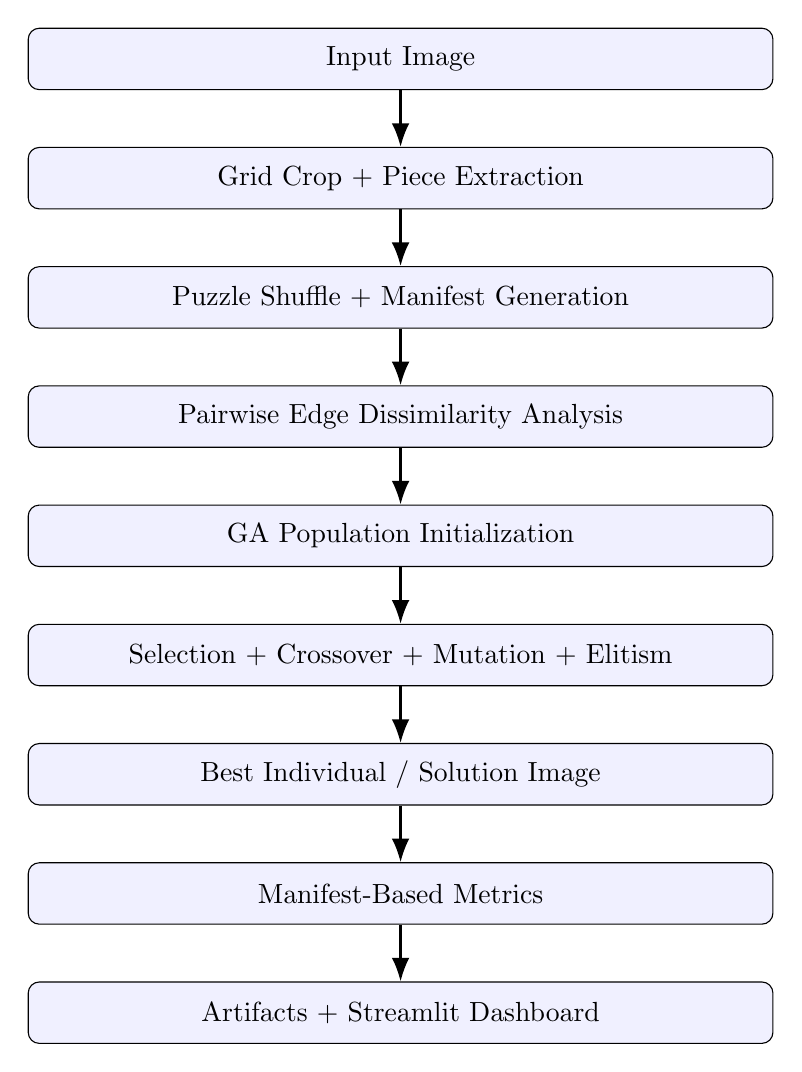
\begin{tikzpicture}[
    node distance=0.72cm,
    box/.style={rectangle, draw, rounded corners, align=center, minimum width=0.78\textwidth, minimum height=0.78cm, fill=blue!6},
    arrow/.style={-{Latex[length=3mm]}, thick}
]
\node[box] (input) {Input Image};
\node[box, below=of input] (crop) {Grid Crop + Piece Extraction};
\node[box, below=of crop] (shuffle) {Puzzle Shuffle + Manifest Generation};
\node[box, below=of shuffle] (analysis) {Pairwise Edge Dissimilarity Analysis};
\node[box, below=of analysis] (population) {GA Population Initialization};
\node[box, below=of population] (evolution) {Selection + Crossover + Mutation + Elitism};
\node[box, below=of evolution] (solution) {Best Individual / Solution Image};
\node[box, below=of solution] (metrics) {Manifest-Based Metrics};
\node[box, below=of metrics] (artifacts) {Artifacts + Streamlit Dashboard};
\draw[arrow] (input) -- (crop);
\draw[arrow] (crop) -- (shuffle);
\draw[arrow] (shuffle) -- (analysis);
\draw[arrow] (analysis) -- (population);
\draw[arrow] (population) -- (evolution);
\draw[arrow] (evolution) -- (solution);
\draw[arrow] (solution) -- (metrics);
\draw[arrow] (metrics) -- (artifacts);
\end{tikzpicture}
\caption{System architecture of the implemented GA jigsaw puzzle workflow.}
\end{figure}

\subsection{Piece Extraction and Puzzle Generation}
The input image is center-cropped so its width and height are divisible by the selected piece size. The valid cropped image is then divided into square pieces. During puzzle creation, the pieces are shuffled using NumPy randomness, and the shuffled pieces are assembled into a puzzle image. The manifest records the mapping from puzzle piece IDs to original piece IDs using fields such as \texttt{version}, \texttt{source\_image}, \texttt{puzzle\_image}, \texttt{piece\_size}, \texttt{rows}, \texttt{columns}, \texttt{cropped\_width}, \texttt{cropped\_height}, and \texttt{puzzle\_to\_original}.

The manifest is one of the main project-specific additions. It allows reliable evaluation after solving without comparing raw image bytes, which can be affected by image encoding and file I/O details.

\subsection{Chromosome Representation}
In the reference paper, a chromosome is represented as an \(N \times M\) matrix of piece IDs \cite{sholomon2016automatic}. In this codebase, an \texttt{Individual} stores a flattened list of pieces along with the number of rows and columns. This is equivalent to a two-dimensional grid because index positions can be mapped back to row and column locations. Each individual also stores a fitness cache and a mapping from piece ID to current index, which supports neighbor lookup during crossover.

\subsection{Edge Dissimilarity and Fitness Calculation}
The project uses edge-color dissimilarity as the fitness basis. For a left-right relation, the right edge of one piece is compared with the left edge of the neighboring piece. For a top-down relation, the bottom edge of one piece is compared with the top edge of the neighboring piece. Color differences are normalized by 255, squared, summed over edge pixels and channels, and square-rooted.

Lower dissimilarity means stronger edge compatibility. The \texttt{Individual.fitness} property accumulates dissimilarities across all adjacent piece pairs and converts the result into a higher-is-better score using \texttt{FITNESS\_FACTOR / accumulated\_dissimilarity}. This follows the same broad principle as the paper: adjacent pieces in the original image should usually have similar colors along their touching edges.

\subsection{Image Analysis Cache}
Computing pairwise edge scores repeatedly would be expensive. The implementation precomputes and stores compatibility information in \texttt{ImageAnalysis.dissimilarity\_measures} and \texttt{ImageAnalysis.best\_match\_table}. The first table stores dissimilarity values for piece pairs and orientations. The second table stores sorted best-match candidates for each piece edge. This cache supports faster fitness evaluation and crossover decisions across generations.

\subsection{Genetic Algorithm Loop}
The \texttt{GeneticAlgorithm} class creates an initial population of \texttt{Individual} objects, analyzes image compatibility, and evolves the population. Each generation preserves elite individuals, selects parents by roulette-wheel selection, creates children by crossover, applies swap mutation according to the mutation rate, and records fitness history. The project tracks \texttt{generations\_completed}, \texttt{termination\_reason}, \texttt{best\_fitness}, and per-generation fitness rows containing \texttt{generation}, \texttt{best\_fitness}, \texttt{average\_fitness}, and \texttt{worst\_fitness}.

The paper reports typical experimental parameters of population size 1000, 100 generations, and mutation rate 0.05 \cite{sholomon2016automatic}. This project uses smaller local defaults, including 20 generations, population 200, and commonly demonstrated mutation rate 0.05. Demo scripts may use population 100 to keep runtime practical.

\subsection{Crossover Operator}
The implemented crossover is inspired by the paper's kernel-growing crossover. It starts from a randomly selected root piece, maintains a growing kernel of placed pieces, tracks taken positions, and adds candidate pieces at available boundaries. The code prefers three kinds of candidate relations:
\begin{enumerate}
    \item A shared parent relation, where both parents agree on the same neighboring piece.
    \item A best-buddy relation, where a parent relation is also a mutual best compatibility match.
    \item A best-match fallback, where the most compatible available piece is selected from image analysis data.
\end{enumerate}

The implementation uses a priority queue to choose candidate placements. It ensures that each piece is used at most once and that the kernel remains within the known puzzle dimensions. This produces a valid complete child arrangement. The position independence of the kernel-growing process is important: a good segment can be inherited as a relative structure even if its final absolute location changes.

\reservedfigure{Paper Figure 3 --- kernel-growing crossover from two parent solutions to a child.}{Kernel-growing crossover concept used as a reference for the project methodology.}

\subsection{Mutation}
The project applies mutation after crossover. If mutation is selected for a child, two random pieces in the individual are swapped. After the swap, the piece mapping is rebuilt and the fitness cache is reset. This differs from the paper's description of mutation inside the crossover procedure, but it serves the same purpose of maintaining search diversity.

\subsection{Termination Conditions}
The GA stops when it reaches the requested maximum number of generations or when the best fitness fails to improve for 10 consecutive generations. The second condition is recorded as \texttt{stagnation}. This prevents unnecessary local runs after the population stops improving.

\subsection{Manifest-Based Evaluation}
The project computes solution metrics using the manifest mapping from shuffled puzzle IDs to original IDs. \texttt{piece\_position\_accuracy} corresponds to direct comparison: the fraction of pieces in their exact original positions. \texttt{adjacency\_accuracy} corresponds to neighbor comparison: the fraction of correct neighboring relationships. The paper explains that neighbor comparison is often more meaningful because a solution can be shifted while preserving many correct local relationships \cite{cho2010probabilistic,sholomon2016automatic}. For that reason, adjacency accuracy is the most useful headline quality metric in this project.

\subsection{Streamlit Visualization Workflow}
The local Streamlit dashboard uses helper functions in \texttt{streamlit\_app/solver\_workflow.py}. It converts uploaded images to BGR format, crops them to a valid puzzle grid, creates a puzzle and manifest in memory, resets the image-analysis cache before each run, runs the GA, collects generation snapshots through a callback, and returns images, metrics, history, snapshots, runtime, and configuration. The dashboard displays upload controls, input preview, run summary cards, tabs for images and metrics, fitness history charts, snapshot galleries, downloads, and logs.

\section{SYSTEM SPECIFICATIONS}
\subsection{Hardware Specifications}
\begin{table}[H]
\centering
\begin{tabular}{ll}
\toprule
\textbf{Component} & \textbf{Specification} \\
\midrule
Operating system & Ubuntu Linux \\
Processor & Intel Core i7-1255U \\
Memory & 16 GB RAM \\
GPU & Not required; CPU-based execution \\
\bottomrule
\end{tabular}
\caption{Hardware specifications for local coursework execution.}
\end{table}

\subsection{Software Specifications}
\begin{table}[H]
\centering
\begin{tabular}{ll}
\toprule
\textbf{Software} & \textbf{Purpose} \\
\midrule
Python 3.x & Solver, CLI, scripts, tests, and dashboard logic \\
LaTeX & Technical report preparation \\
Git & Version control \\
Ubuntu shell & Local command execution \\
\bottomrule
\end{tabular}
\caption{Software specifications.}
\end{table}

\subsection{Tools and Libraries Used}
\begin{longtable}{>{\raggedright\arraybackslash}p{0.28\textwidth}>{\raggedright\arraybackslash}p{0.62\textwidth}}
\toprule
\textbf{Tool or Library} & \textbf{Use in Project} \\
\midrule
NumPy & Array operations, shuffling, and numerical calculations. \\
OpenCV & Image reading, writing, BGR image handling, and piece-size detection support. \\
Pillow & Image conversion and PNG byte generation for dashboard downloads. \\
Matplotlib & Fitness plot generation in CLI workflows. \\
Click & Command-line interface for \texttt{gaps create}, \texttt{gaps run}, and \texttt{gaps baseline}. \\
Streamlit & Local visualization dashboard. \\
Pytest & Automated tests for workflow helpers, manifest metrics, and solver behavior. \\
\bottomrule
\end{longtable}

The main dependency metadata is stored in \texttt{pyproject.toml}. The Streamlit runtime dependencies are listed in \texttt{streamlit\_app/requirements.txt}.

\section{Experimental Results}
\subsection{Literature Benchmark Context}
The following values are literature results from Sholomon et al. \cite{sholomon2016automatic}. They are included to explain the research context and are not claimed as this project's local results.

\reservedfigure{Paper Figure 4 --- large puzzle reconstruction progress across generations.}{Literature example of generation-wise improvement in GA-based jigsaw solving.}
\reservedwide{Paper Table 2 --- neighbor-comparison benchmark results.}{Literature benchmark results under neighbor comparison.}

\begin{table}[H]
\centering
\begin{tabular}{rccp{0.26\textwidth}}
\toprule
\textbf{Puzzle Pieces} & \textbf{Neighbor Avg. Best} & \textbf{Neighbor Avg. Avg.} & \textbf{Notes} \\
\midrule
432 & 96.16\% & 95.70\% & Smaller benchmark \\
805 & 96.26\% & 95.85\% & Smaller benchmark \\
10,375 & 98.47\% & 98.36\% & Large puzzle set \\
22,755 & 96.40\% & 96.19\% & Very large puzzle set \\
30,745 & 93.40\% & 93.27\% & Largest paper benchmark \\
\bottomrule
\end{tabular}
\caption{Selected neighbor-comparison results reported in the reference paper.}
\end{table}

\reservedwide{Paper Table 6 --- average runtime table.}{Literature runtime scaling for single-threaded and multi-threaded GA runs.}

\begin{table}[H]
\centering
\begin{tabular}{rll}
\toprule
\textbf{Puzzle Pieces} & \textbf{Runtime} & \textbf{Mode} \\
\midrule
432 & 48.73 sec & Single-threaded \\
805 & 116.18 sec & Single-threaded \\
10,375 & 3.21 hr & Single-threaded \\
22,755 & 13.19 hr & Single-threaded \\
22,755 & 3.43 hr & Multi-threaded \\
30,745 & 6.51 hr & Multi-threaded \\
\bottomrule
\end{tabular}
\caption{Selected runtime values reported in the reference paper.}
\end{table}

\subsection{Local Demonstration Setup}
A representative local demonstration can use the following configuration:
\begin{table}[H]
\centering
\begin{tabular}{ll}
\toprule
\textbf{Item} & \textbf{Value} \\
\midrule
Image & \texttt{images/messi.jpg} \\
Piece size & 64 pixels \\
Cropped dimensions & \(960 \times 512\) \\
Grid & \(8 \times 15\) \\
Total pieces & 120 \\
Generations requested & 20 \\
Population & 100 \\
Mutation rate & 0.05 \\
Seed & 42 \\
Snapshot interval & 1 or 5 \\
Hardware & Ubuntu Linux, Intel i7-1255U, 16 GB RAM \\
\bottomrule
\end{tabular}
\caption{Representative local demonstration setup.}
\end{table}

\subsection{Local Solver Output}
In a sample deterministic local run, the solver reconstructed most piece relationships correctly and terminated early due to stagnation. The sample output was:
\begin{table}[H]
\centering
\begin{tabular}{ll}
\toprule
\textbf{Metric} & \textbf{Value} \\
\midrule
Generations completed & 13 \\
Termination reason & Stagnation \\
Piece-position accuracy & 97.50\% \\
Correct positions & 117/120 \\
Adjacency accuracy & 97.24\% \\
Correct adjacencies & 211/217 \\
Best fitness & 6.887182 \\
Runtime & Approximately 2.88 seconds \\
\bottomrule
\end{tabular}
\caption{Sample local solver result for a deterministic coursework-scale run.}
\end{table}

These results should be interpreted as one local demonstration, not as a guarantee for all images or settings. The final quality depends on the image content, piece size, population, generation count, mutation rate, and random seed.

\subsection{Fitness History and Convergence}
The project records best, average, and worst fitness for every completed generation. The CLI can export this history to CSV and produce a Matplotlib fitness plot. The Streamlit dashboard displays the same data as a line chart and table. If the best fitness does not improve for 10 generations, the solver can terminate early due to stagnation.

\subsection{Snapshot-Based Visual Progress}
Generation snapshots show the best individual at selected points during evolution. The CLI writes snapshots to a directory when \texttt{--snapshots-dir} is provided. The Streamlit workflow stores snapshots in memory and displays them as a gallery with per-snapshot PNG downloads.

\reservedfigure{Paper Figure 5 --- shifted solutions with low direct accuracy but high neighbor accuracy.}{Example showing why neighbor/adjacency accuracy is more meaningful than direct position accuracy.}

\subsection{Experiment Runner}
The experiment script creates one base puzzle and manifest, then evaluates a small grid of GA configurations. The current script uses \texttt{images/baboon.jpg}, seed 42, piece size 64, generations \([10, 20]\), population \([50]\), and mutation rates \([0.0, 0.05, 0.1]\). It writes \texttt{outputs/experiments/results.csv} with fields such as run ID, seed, generations, population, mutation rate, completed generations, best fitness, termination reason, runtime, piece-position accuracy, adjacency accuracy, manifest path, history path, and solution path.

\section{Project Screenshots}
The following reserved boxes are for screenshots that can be inserted later.

\reservedfigure{Screenshot 1: Streamlit upload and local solver controls.}{Streamlit upload and local solver controls.}
\reservedfigure{Screenshot 2: Input preview with original size, cropped size, grid, and piece count.}{Input preview with image size and puzzle grid details.}
\reservedfigure{Screenshot 3: Run Summary and Overview tab.}{Run Summary and Overview tab.}
\reservedfigure{Screenshot 4: Images tab showing cropped original, shuffled puzzle, GA solution, and comparison image.}{Images tab showing puzzle reconstruction outputs.}
\reservedfigure{Screenshot 5: Metrics tab showing piece-position and adjacency accuracy.}{Metrics tab showing manifest-based solution quality.}
\reservedfigure{Screenshot 6: Fitness History tab showing line chart and table.}{Fitness History tab showing convergence information.}
\reservedfigure{Screenshot 7: Snapshots tab showing generation snapshots.}{Snapshots tab showing generation-wise visual progress.}
\reservedfigure{Screenshot 8: Downloads and Log tab.}{Downloads and Log tab.}
\reservedfigure{Screenshot 9: CLI run output and generated artifacts directory.}{CLI run output and generated artifacts directory.}

\section{Limitations}
The project supports only Type-1 puzzles. Pieces must be square, fixed in orientation, and non-overlapping. There is no handling for missing pieces, rotated pieces, unknown orientations, or unknown puzzle dimensions beyond determining the grid after cropping.

Runtime grows as the piece count, population size, and generation count increase. Larger puzzles require more pairwise compatibility analysis and more crossover operations per generation. The Streamlit dashboard stores snapshots in memory, so high snapshot counts can increase memory use during a run.

The edge-color dissimilarity fitness can fail on smooth or repetitive image regions such as sky, water, grass, walls, or other low-texture areas. In such regions, incorrect neighbors may have very similar edge colors. Fitness improvement therefore does not always guarantee a human-perfect reconstruction. Direct comparison can also be misleading for shifted solutions, which is why adjacency accuracy is emphasized.

This project demonstrates a local coursework-scale solver and does not reproduce the very large benchmark scale of the reference paper.

\reservedfigure{Paper Figure 5 --- shifted solutions and neighbor comparison.}{Shifted solution example illustrating the limitation of direct position accuracy.}

\section{Conclusion}
This project successfully implements a GA-based Type-1 jigsaw puzzle solver and connects research ideas from Sholomon et al. to a working Python system. The solver uses edge-dissimilarity fitness, image-analysis caching, roulette selection, elitism, kernel-growing crossover, mutation, and termination tracking. Around the solver, the project provides a CLI workflow, deterministic puzzle generation, manifest-based evaluation, random baselines, fitness history, plots, snapshots, an experiment runner, and a local Streamlit dashboard.

The most important evaluation feature is the manifest-based metric design. Piece-position accuracy gives direct placement correctness, while adjacency accuracy captures neighbor relationships and is usually the more meaningful headline metric for jigsaw reconstruction. Overall, the project demonstrates search, optimization, fitness evaluation, visualization, artifact generation, and experiment tracking in a clear coursework-oriented implementation.

\section{References}
\bibliographystyle{plain}
\bibliography{references}

\end{document}
